\documentclass[Space3_Assign1.tex]{subfiles}

\begin{document}
\newpage
\section{Orbital Determination}

\subsection{Introduction}
Three networks are used to communicate with the Van Allen Probes [3]. The main communications ground station is at the Applied Physics Laboratory in Washington, USA. The LLH coordinates are 39.10N 76.53W 140 m above mean seal level. [4] \\
For backup, the satellite communicates with the United Space Network using the Near Earth Network with ground stations in Hawaii(19.0N 155.6W 367m) and Australia. The data rates that can be achieved with this network is high enough to gather scientific data from the probe. Also as a backup, the NASA program Space Network is used for monitoring data, which relays through geosynchronous Tracking and Data Relay Satellites (TDRS). The TLEs are collected at approximately the same point in the orbit, at a mean anomaly of 345$^{\circ}$. The Van Allen Probes have two S-band RF antennas and use RF doppler data acquired for ground contacts.\\
For the noise analysis, 
Nominal uplink 20dB, minimum downlink margin 3dB

\subsection{Methodology}
The perturbation model from Question 2 was used to simulate the orbit.
\begin{figure}[h!]
\centering
\caption{}
\label{fig:Q3_gnd}
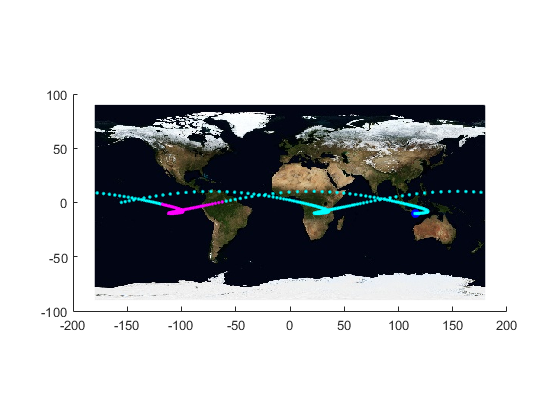
\includegraphics[width=1\linewidth]{Q3_gnd}
\end{figure}

\begin{figure}[h!]
\centering
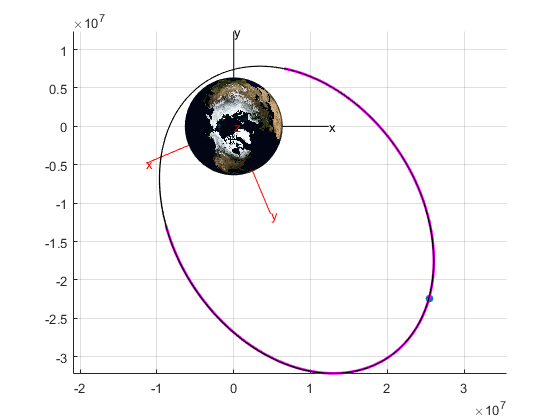
\includegraphics[width=0.7\linewidth]{Q3_sim_top}
\caption{Pink highlights when the satellite was in view of the ground station.}
\label{fig:Q3_sim_top}
\end{figure}

\subsection{Results/Discussion}
The main ground station in Washington USA was simulated. Therefore the ground station location was 39.10N 76.53W 140 m and a minimum elevation of 10 degrees from the horizon was implemented. This is so that any trees or small terrain fluctuations are accounted for.





\subsubsection{HG - no noise}
\begin{figure}[h!]
\centering
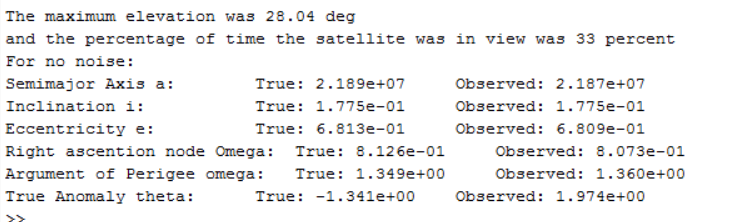
\includegraphics[width=1\linewidth]{nonoise}
\caption{HG analysis no noise}
\label{fig:nonoise}
\end{figure}


\subsubsection{Noise Analysis}
\begin{figure}[h!]
\centering
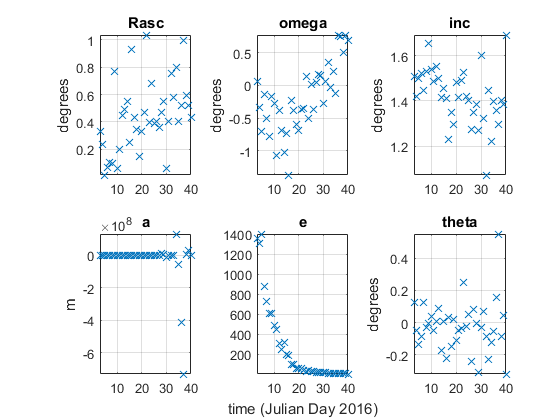
\includegraphics[width=1\linewidth]{NOISE}
\caption{Noise analysis *Note x axis label wrong 'Sound to Noise ratio dB'}
\label{fig:NOISE}
\end{figure}

\end{document}